Um in die Einstellungen für die Monitore zu gelangen, klicken Sie im \enquote{Data-Input-Menü} auf den Punkt \enquote{Monitore verwalten} (siehe Abbildung \ref{menu-data-input}).\\
\\
\begin{figure}[H]
\centering
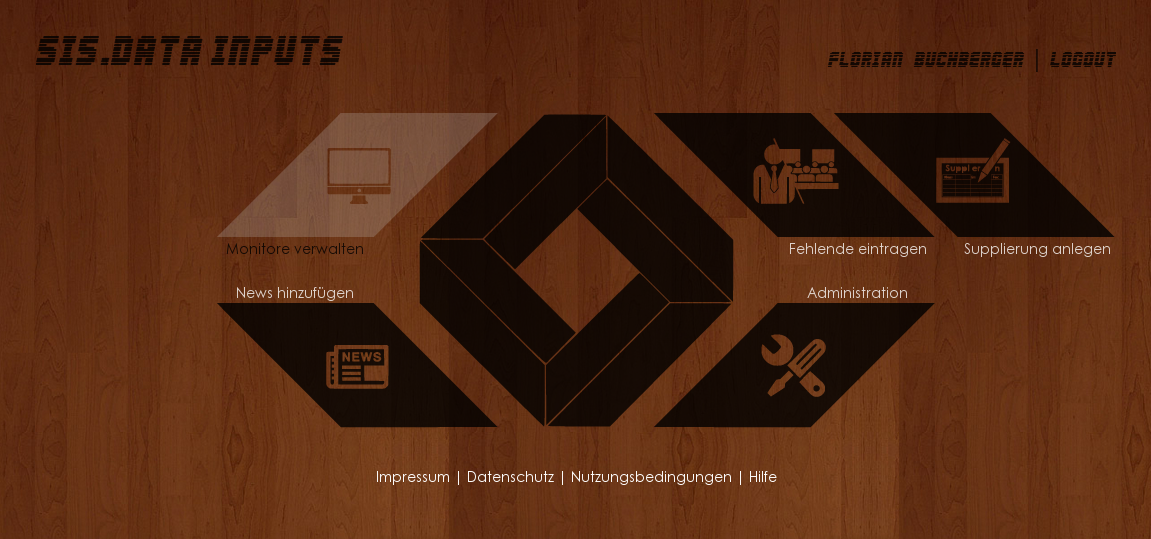
\includegraphics[keepaspectratio=true, width=14cm]{images/screenshots/data-inputs.png}
\label{menu-data-input}
\caption{Data-Input-Menü}
\end{figure}
Nach dem Öffnen der Seite werden oben im Fenster die aktiven Monitore aufgelistet. Darunter sind die Einstellungen zu finden.\\
\\
\begin{figure}[H]
\centering
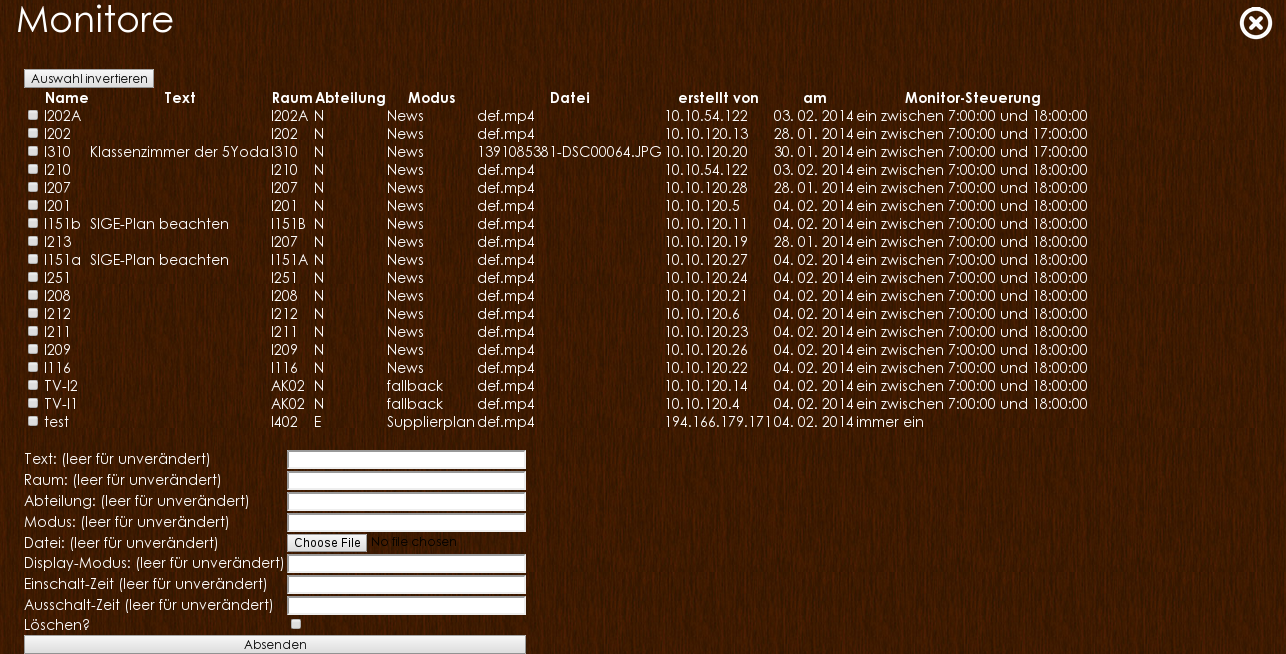
\includegraphics[keepaspectratio=true, width=14cm]{images/screenshots/monitors.png}
\label{monitors}
\caption{Monitor-Einstellungen}
\end{figure}
Die Monitore, deren Einstellungen verändert werden sollen, müssen mit einem Klick auf die Checkbox links neben der Anzeige ausgwählt werden. Es können mehrere ausgewählt werden. Mit dem Button \enquote{Auswahl invertieren} werden alle gesetzten Checkbox rückgesetzt, und umgekehrt.
\\
\subsection{Hinzufügen}

Ein neuer Monitor kann nicht über das Web-Interface hinzugefügt werden, die Monitore registrieren sich selbstständig am Server. Nach der Registrierung stehen sie zur Verwaltung zur Verfügung.

\subsection{Entfernen}

Um einen Monitor aus der Liste der aktiven Monitore zu entfernen, wähle den jeweiligen Monitor über die Checkbox aus, setze die \enquote{Löschen?}-Checkbox und klicke auf \enquote{Änderungen anwenden}.

\subsection{Text verändern}

Der Text, der am linken unterem Eck des Monitors kann über das Eingabefeld \enquote{Text} geändert werden. Wird das Feld leer gelassen, so wird der alte Wert beibehalten.\\
\textit{Achtung:} Leerzeichen werden nicht als leer erkannt.

\subsection{Raum verändern}

Für die Darstellung des Stundenplanes des jeweiligen Raumes wird jedem Monitor ein Raum zugeordnet. Diese Einstellung kann über das Eingabefeld \enquote{Raum} angepasst werden. Durch Doppelklick auf das Eingabefeld öffnet sich - sofern der verwendete Browser diese Funktion unterstützt - ein Menü, indem 